\chapter{Identificação do Túnel de Ar} \label{cap4}

Neste capítulo, será explicada a identificação do sistema do túnel de ar. Para fazer a identificação caixa-preta de um sistema é necessário fazer um estudo prévio do funcionamento dele, conhecer entradas e saídas, obter um modelo matemático se possível, mesmo sem ter todos os parâmetros.
\section{Escolha de estrutura}
A escolha da estrutura para identificar um sistema pode ser feita a partir de um modelagem prévia do sistema \commentib{Isso é parcialmente verdade, o conhecimento empírico da modelagem fenomeológica pode fornecer pistas sobre a estrutura, mas existem outros métodos que valem a pena ao menos serem citados, tais como análise de função de autocorrelação} , mas, em alguns casos a modelagem não é suficiente para obter um modelo adequado. O nosso modelo apresenta uma interação entre o ar e a bola que é difícil de ser modelado, quando uma esfera gira ela interage com o ar criando um fenômeno chamado efeito Magnus \cite{briggs1959}, esse fenômeno influencia no movimento da esfera fazendo ela se mover de uma forma previsível, no entanto, como o giro é causado pelo fluxo de ar e é possível observar que ele constantemente muda de direção, não podemos modelar o sistema de forma satisfatória. Então, precisamos explorar um método diferente para escolher a estrutura do sistema.

\subsection{Mínimos Quadrados}\label{s:4mq}

A identificação por Mínimos Quadrados gera um sistema do tipo ARX como visto na equação \eqref{eq:ARXModel}. A escolha da estrutura neste caso se dá escolhendo uma quantidade de regressores da saída e uma quantidade de regressores da entrada. 


Para a escolha da estrutura do modelo do sistema foi feito o seguinte procedimento:
\begin{enumerate}
	\item Escolher uma quantidade de regressores de $y$
	\item Escolher uma quantidade de regressores de $u$
	\item Fazer a identificação por Mínimos Quadrados com os regressores de $y$ e $u$
	\item Analisar a autocorrelação dos resíduos $\xi=y-\Psi \hat{\theta}$
\end{enumerate}

Este procedimento foi repetido para valores de 1 a 10 para ambos os regressores para escolhermos quantos zeros e polos precisamos para uma estrutura que tem a seguinte forma:

\begin{equation}
Y[k]=\dfrac{A[k]}{B[k]}
\end{equation}
\begin{equation}
A[k]=a_1 U[k-1]+a_2 U[k-2]+ \dots + a_n U[k-n]
\end{equation}
\begin{equation}
B[k]=b_1 Y[k-1]+b_2 Y[k-2]+ \dots + b_m Y[k-m]
\end{equation}

Onde n é o número de zeros e m é o número de polos. Ao final se identificou que a melhor ordem para os regressores foi com 9 polos e 8 zeros.

\subsection{Subespaços}\label{s:4subespacos}
A identificação por Subespaços gera um sistema em espaço de estados como visto na equação \eqref{eq:ss}. Neste tipo de identificação a escolha da estrutura é feita decidindo a ordem do sistema e a ordem da matriz em blocos de Hankel. E similarmente ao procedimento feito na seção \ref{s:4mq} foram variadas as ordens do sistema e da matriz em blocos de Hankel.
Foi escolhida ordem 3 para o sistema e ordem 15 para a matriz em blocos de Hankel usada para identificar o sistema. Vemos na figura \ref{fig:autocorrelacao315} a auto correlação dos resíduos do sistema identificado.



\section{Experimento}\label{s:4experimento}
O experimento para identificação precisa de um sinal adequado para que a resposta à ele consiga mostrar a dinâmica do sistema. Para tanto foi gerado um sinal PRBS (sinal binário pseudo aleatório) que é suficientemente adequado para extrair a dinâmica do sistema. O sinal é aplicado ao sistema através do Arduino e os sinais são medidos com um tempo de amostragem de 50 ms.
\begin{figure}[H]
	\centering
	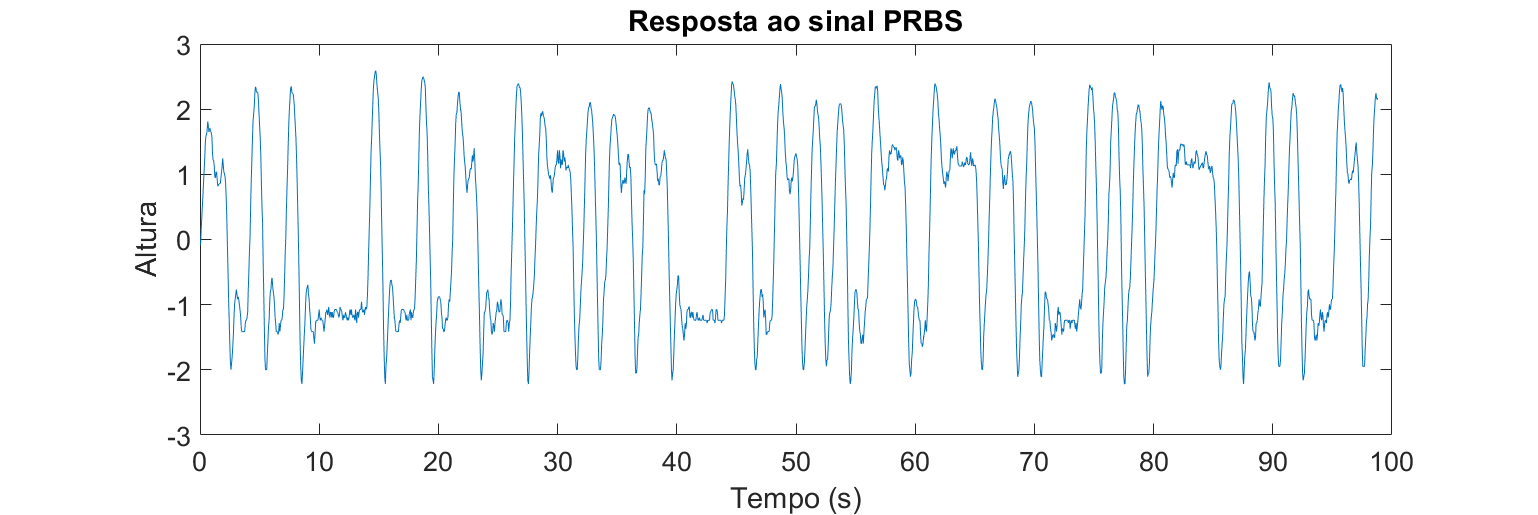
\includegraphics[width=1.1\linewidth]{sinalprbsid}
	\caption[Gráfico da saída PRBS]{Gráfico da saída ao aplicar o sinal PRBS com tempo de amostragem de 50ms}
	\label{fig:sinalprbsid}
\end{figure}

A figura \ref{fig:sinalprbsid} mostra a resposta do sistema ao sinal PRBS que foi aplicado ao sistema, podemos ver seções do teste onde o sinal possibilitou que o sistema tivesse algum tempo para estabilizar como em torno dos 10 e 80 segundos,e em outros o sistema é posto em movimento.

\section{Estimação}\label{s:4estimacao}

Com a resposta ao sinal PRBS em mãos podemos identificar o sistema. Usando o método dos mínimos quadrados e o método de identificação por subespaços.

\subsection{Mínimos Quadrados}\label{s:4estmq}
Para fazer a identificação por mínimos quadrados geramos a matriz de regressores $\psi$ da equação \eqref{eq:regressores} e usamos a equação \eqref{eq:MQ} para obter os coeficientes dos regressores. Obtemos um sistema com o seguinte modelo ARX:

\begin{equation}
\begin{matrix}
a_1= -0.004773 &
a_2= -0.002941&
a_3=  0.01512 \\
a_4=  0.01026 &
a_5=  0.04134 &
a_6=  0.01709\\
a_7=  0.003757 &
a_8=  0.0386
\end{matrix}
\end{equation}
\begin{equation}
\begin{matrix}
b_1= -1.463&
b_2=  0.6593&
b_3= -0.4703\\
b_4=  0.3195&
b_5=  0.1436&
b_6= -0.1106\\
b_7=  0.07184&
b_8= -0.0766& 
b_9=  0.02136
\end{matrix}
\end{equation}

\subsection{Subespaços}\label{s:4estsub}

Para identificar o sistema usando subespaços utilizamos o algoritmo mostrado na seção \ref{s:subalgoritmos} com uma matriz em blocos de Hankel de ordem 15 para encontrar um sistema de ordem 3. Identificamos o seguinte modelo com o formato da equação \eqref{eq:ss}:

\begin{equation}
A=\begin{bmatrix}
0.9761  &  0.1933 &  -0.0438\\
-0.1817  &  0.9841  & -0.1489\\
0.0840  &  0.3107  &  0.6994
\end{bmatrix}
\end{equation}

\begin{equation}
B=\begin{bmatrix}
0.1466\\
0.2515\\
0.8460
\end{bmatrix}
\end{equation}
\begin{equation}
C=\begin{bmatrix}
-1.0104 &  -0.3354 &   0.2496
\end{bmatrix}
\end{equation}
\begin{equation}
D=\begin{bmatrix}
0.0010
\end{bmatrix}
\end{equation}

\section{Validação}\label{s4:val}
Ao identificar um sistema precisamos validar o modelo obtido para garantir que ele é adequado para representar o sistema real. Para isso fazemos uma análise da auto correlação dos resíduos $\xi=y-\Psi \hat{\theta}$ para o ARX e $\xi=y-y_{sim}$ para o espaço de estados. Como vemos nas figuras \ref{fig:autocorrelacao98} e \ref{fig:autocorrelacao315} os resíduos do modelo ARX são muito menos correlacionados do que os do modelo em espaço de estados. Isso acontece porque para o modelo ARX estamos analisando os seus regressores com a matriz $\Psi$ que os gera, o que retorna uma resposta muito mais próxima do sistema. Já para o espaço de estados estamos analisando a simulação do sistema, que apresenta pequenas diferenças em relação ao sistema real, como a ausência de ruído.


Olhamos também a resposta ao degrau do sistema, figuras \ref{fig:respostadegrauarx} e \ref{fig:respostadegrausub}, e vemos que para os dois sistemas identificados ela tem uma oscilação similar ao sistema real. Concluímos, através da análise da auto correlação dos resíduos e da análise da resposta ao degrau dos sistemas identificados, que os modelos são adequados para mostrar o funcionamento do sistema.

\begin{figure}[H]
	\centering
	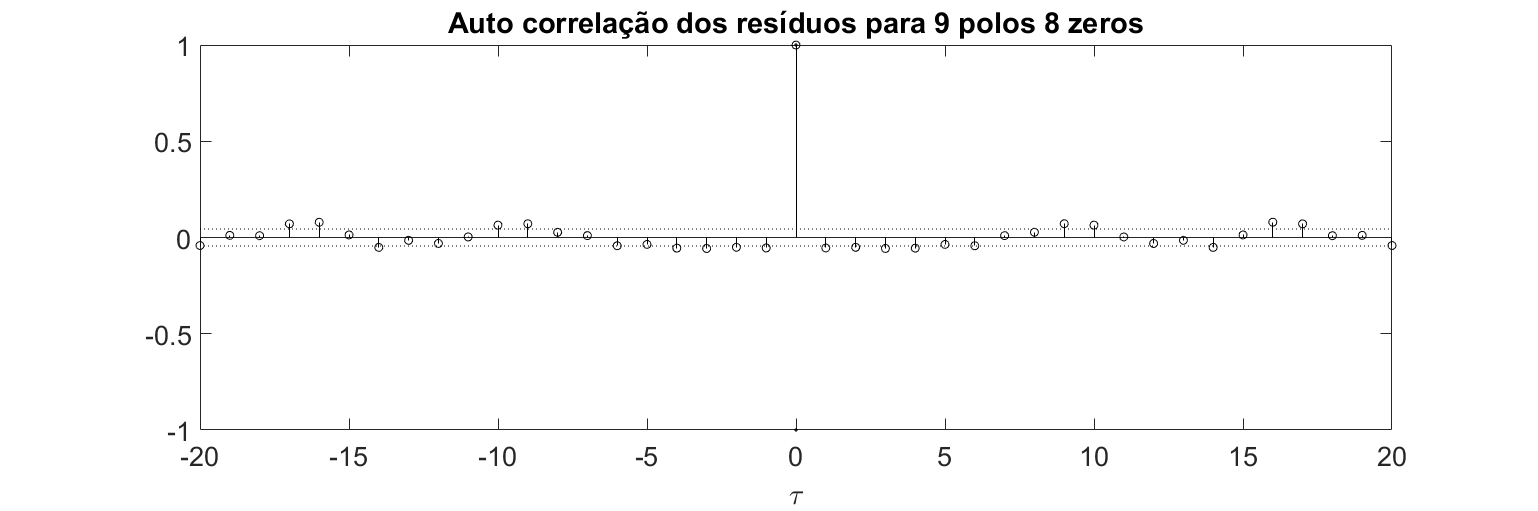
\includegraphics[width=1.1\linewidth]{autocorrelacao98}
	\caption[Autocorrelação dos resíduos para sistema com 9 polos e 8 zeros]{Autocorrelação dos resíduos para sistema com 9 polos e 8 zeros}
	\label{fig:autocorrelacao98}
\end{figure}

\begin{figure}[H]
	\centering
	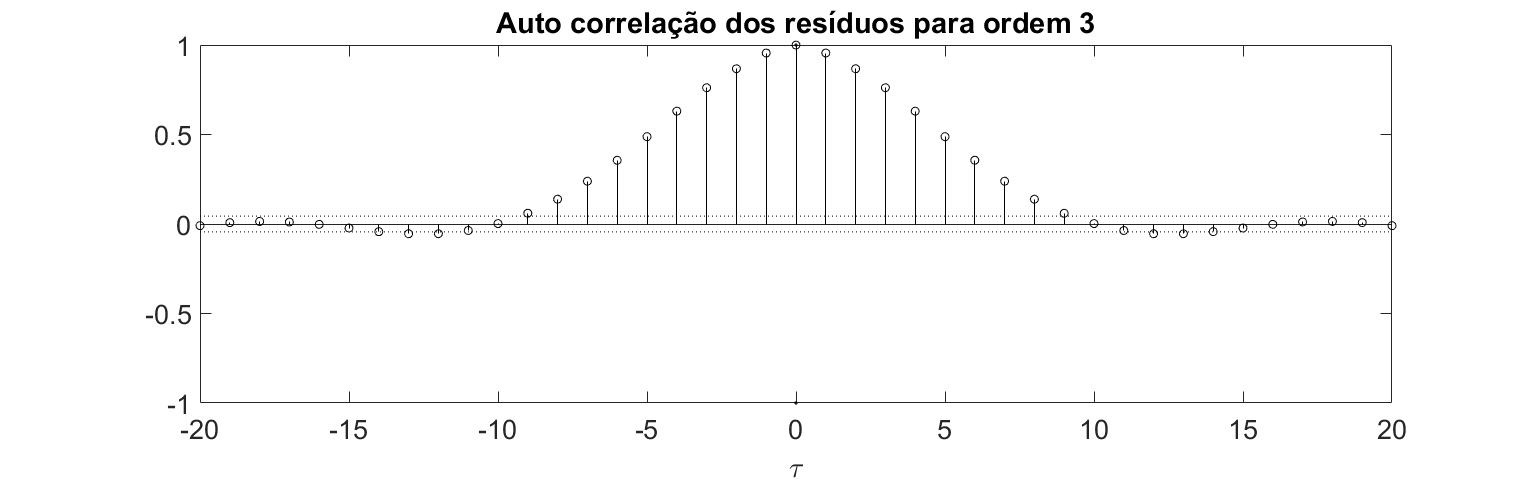
\includegraphics[width=1.1\linewidth]{autocorrelacao315}
	\caption[Autocorrelação dos resíduos para sistema de ordem 3]{Autocorrelação dos resíduos para sistema de ordem 3 identificado com matriz em blocos de Hankel ordem 15}
	\label{fig:autocorrelacao315}
\end{figure}

\begin{figure}[H]
	\centering
	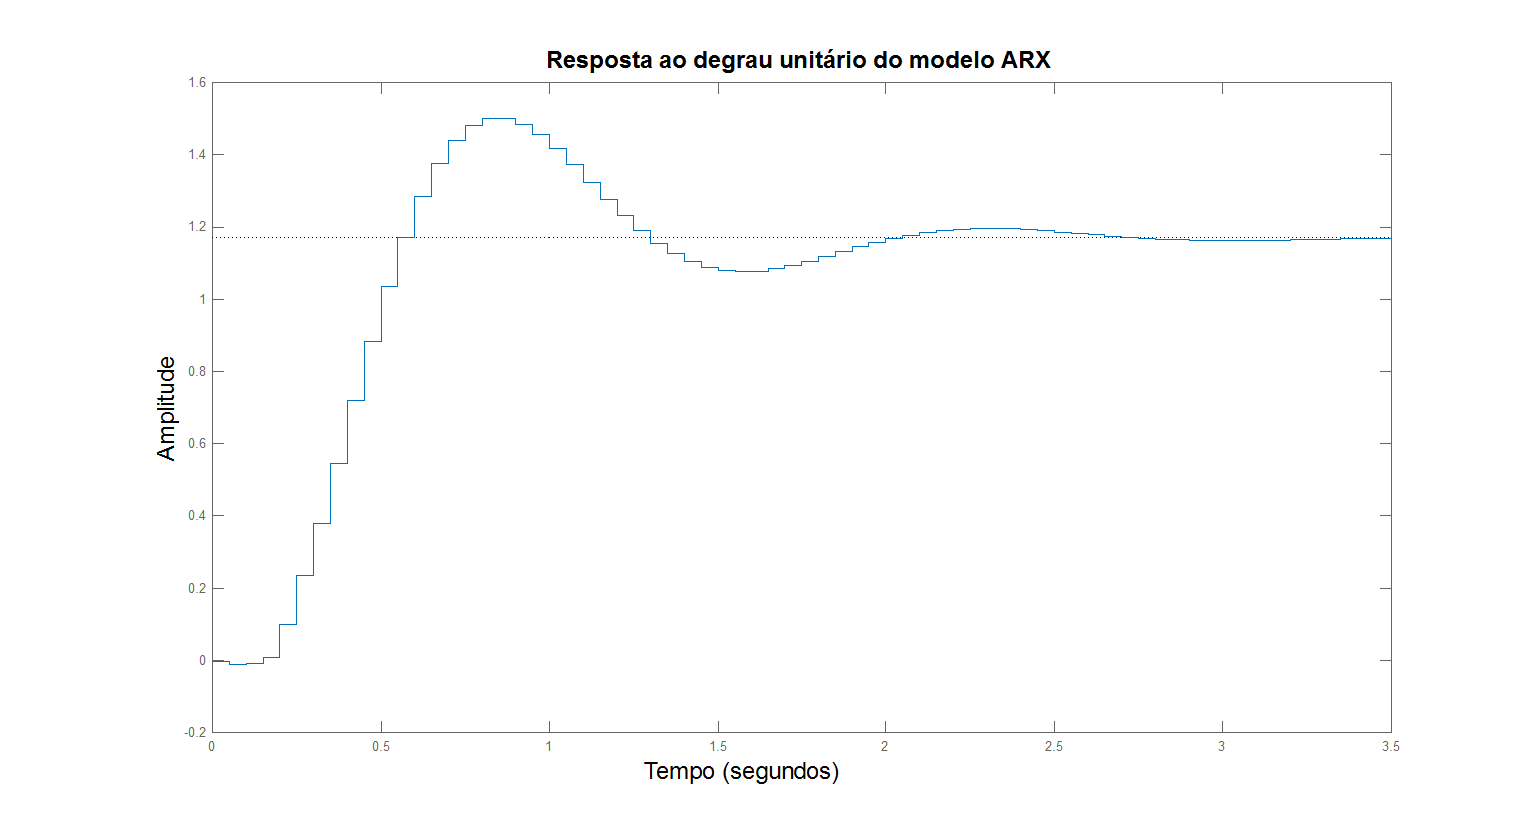
\includegraphics[width=1\linewidth]{respostadegrauarx}
	\caption[Resposta ao degrau do modelo ARX]{Resposta ao degrau unitário do modelo ARX identificado}
	\label{fig:respostadegrauarx}
\end{figure}

\begin{figure}[H]
	\centering
	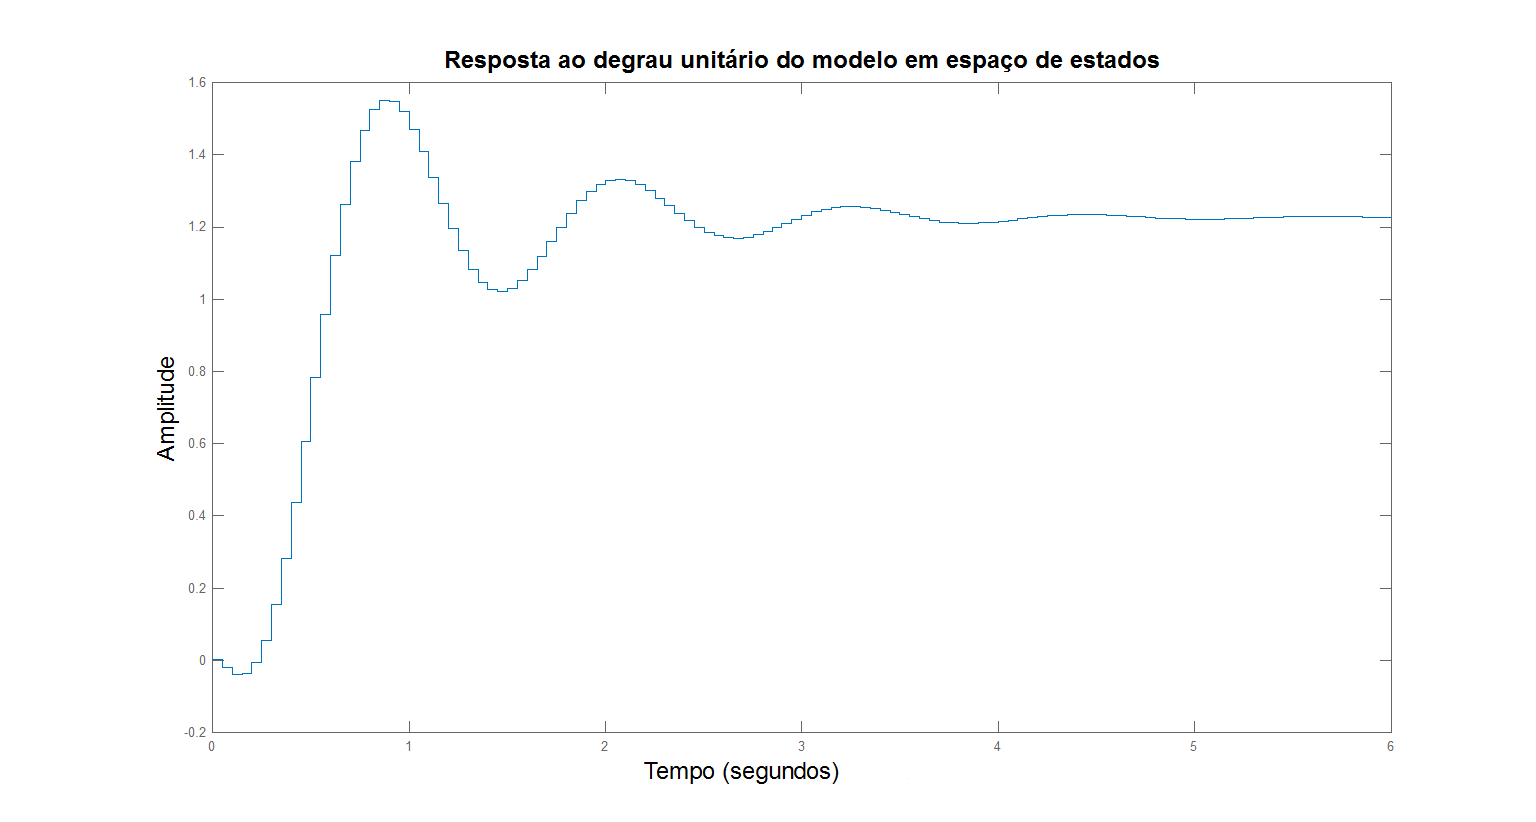
\includegraphics[width=1\linewidth]{respostadegrausub}
	\caption[Resposta ao degrau do modelo em espaço de estados]{Resposta ao degrau unitário do modelo em espaço de estados identificado}
	\label{fig:respostadegrausub}
\end{figure}



% Fim Capítulo